%# -*- coding: utf-8-unix -*-
%%==================================================
%% chapter01.tex for SJTU Master Thesis
%%==================================================

%\bibliographystyle{sjtu2}%[此处用于每章都生产参考文献]
\chapter{语言模型}
\label{chap:lm}




语言模型通常被用来解决这类问题:语音识别、机器翻译、音字转换、自动文摘、问答系统等。
在自动语音识别(ASR)领域中,语言模型扮演着十分重要的角色。
本文介绍的重点主要围绕语言模型在语音识别中的优化展开。


\section{语言模型在语音识别(ASR)中的作用} 
%如图~\ref{fig:SDS}所示,这是一个典型的口语对话系统,其中各个模块依次传递信息。按照图中箭头方向的一个回环就是一轮对话,其中包括:
一轮人机交互是从语音到文字的语音识别、从文字到语义的口语语义理解、从语义输入到反馈的对话状态跟踪和管理模块、从语义反馈又到文本的自然语言生成、从文本回到语音的语音合成。

%\begin{figure}[htbp!]
%\centering
%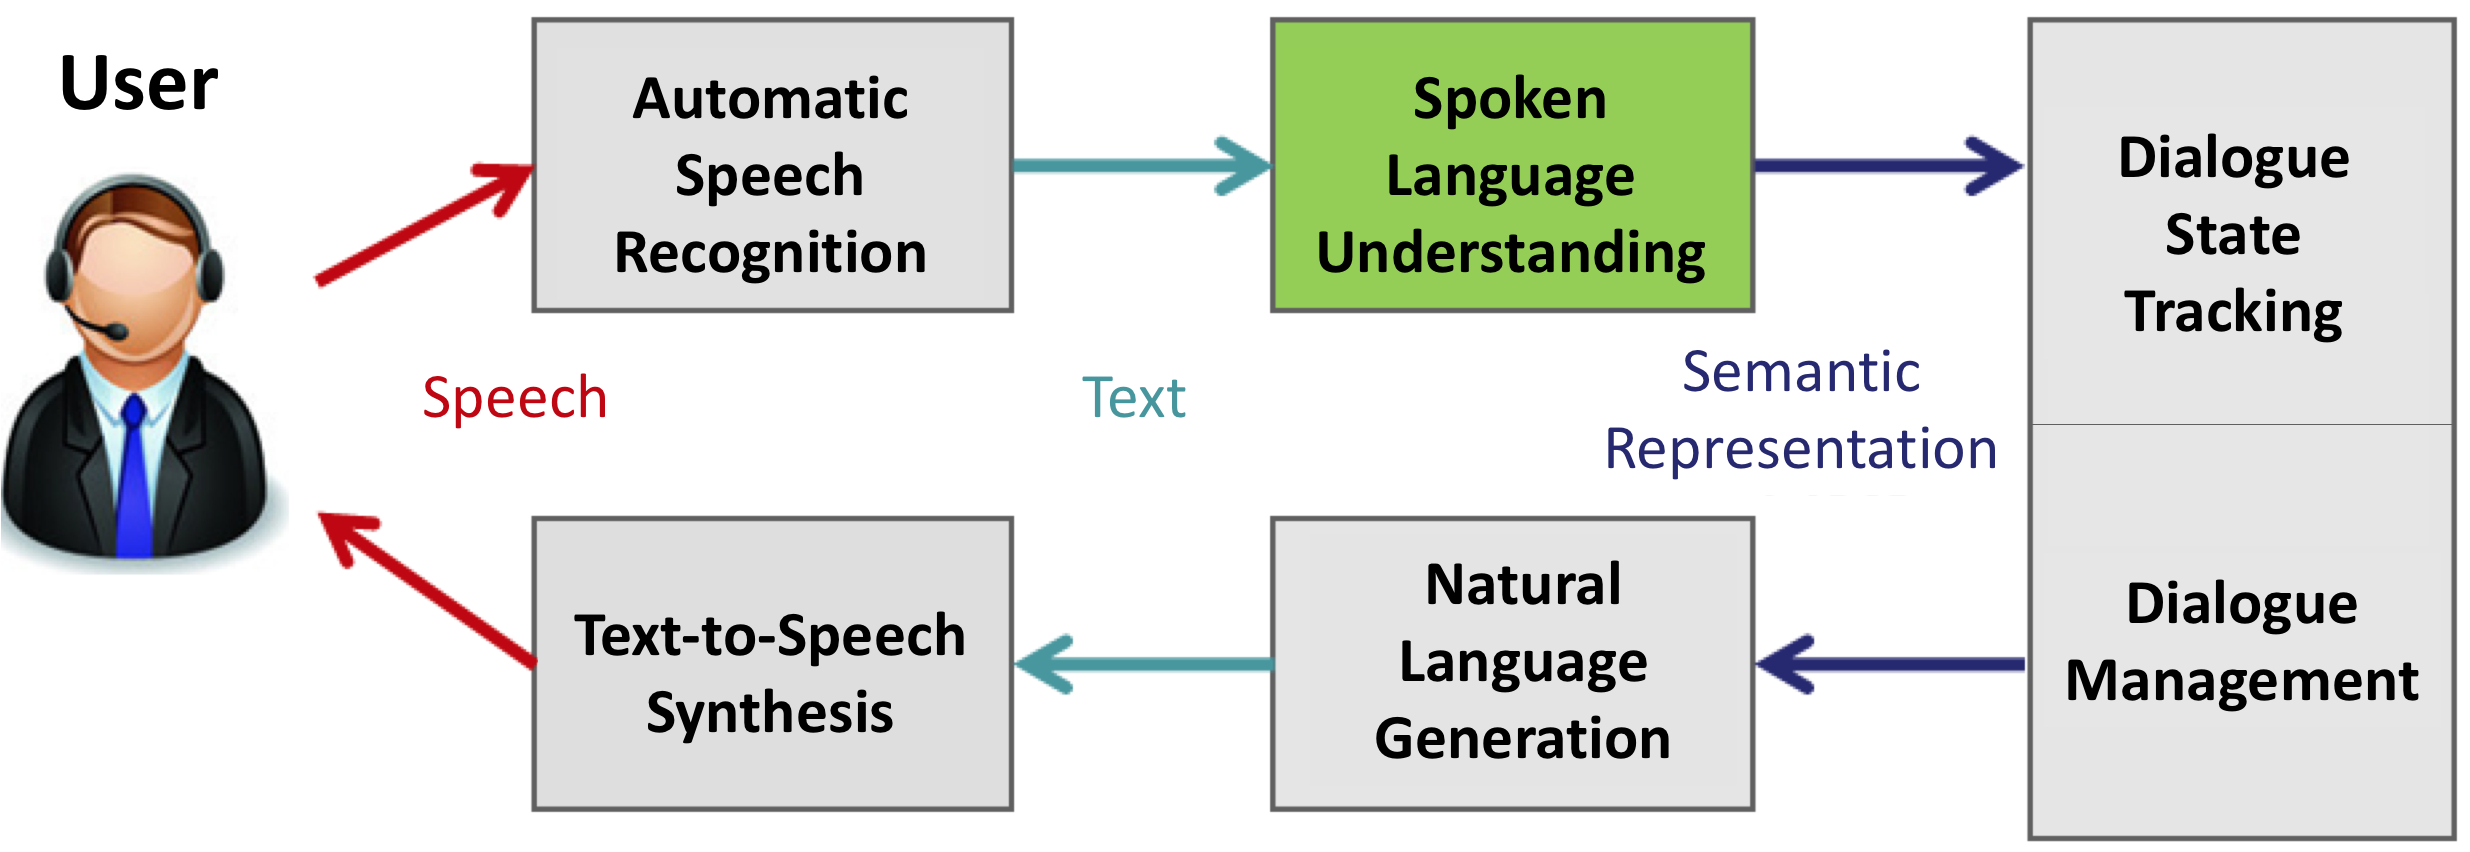
\includegraphics[width=1.0\textwidth]{struclm/SDS}
%\caption{在口语对话系统中的口语语义理解}
%\label{fig:SDS}
%\end{figure}

语音识别(Automatic Speech Recognition, ASR)模块是上述一轮对话流程中的第一个组件,而且它的输出被用于口语语义理解的输入信息。语音波形经过前端的特征提取和各种预处理后,通过识别阶段,得到含有识别结果的文本输出,声学模型和语言模型就是合作完成这个识别功能的。语音识别的过程是将声学信号的特征序列($O$)映射成词序列($W$),如下公式~\ref{equ:asr-model}所示:
\begin{equation}
\hat{W} = \mathop{\text{arg max}}_{W}P(W|O) \ \varpropto\ P(O|W)P(W)
\label{equ:asr-model}
\end{equation}

公式~\ref{equ:asr-model}最后分成了两部分$P(O|W)$和$P(W)$:其中$P(O|W)$代表的是声学模型(Acoustic Model, AM),将声学信号转成所有可能的词序列;$P(W)$代表语言模型(Language Model, LM),其作用是在声学模型产生的所有可能的词序列中选择尽可能符合自然语言的词序列。


通俗的说,声学模型将语音的数字信号识别成具体的词和读音,然后输入到语言模型中,形成识别结果。
例如有个句子是“我很酷”,当语言模型已经识别出来前两个字是“我”和“很”时,当输入第三读音是ku时,博大精深的汉字库并没有办法确定是“酷”还是“苦”或者是其它词,这时语言模型需要给出的是当历史信息是某一确定句子时,后面一个词的出现概率是多少,然后通过某个词在某一特定历史信息下出现的概率得到一段文字(句子)出现的概率,如公式(\ref{eq:psen})所示
\begin{equation}
	\label{eq:psen}
   	P(s) = P({w_1})*P({w_2}|{w_1})*P({w_3}|{w_1}{w_2})*...*P({w_m}|{w_1}...{w_{m - 1}}) = \prod\limits_{i = 1}^m {P({w_i}|{w_1}...{w_{i - 1}})} 
%% 	P(s) = P(w_2)*P(w_2|w_1)P(w_3|w_{1}w_{2})*...*P(w_{m}...w_{m-1}) = \prod_{i=1}^{m}{p(w_{i}|w_{1}...w{i-1})}
\end{equation}

$w_{i}$可以是字、词、短语或词类等,称为统计基元,$w_{i}$ 的概率由$w_1$,……,$w_{i-1}$决定,由特定的$w_1$,$...$,$w_{i-1}$构成的序列成为$w_i$的历史。
下文中我们统称$w$为单词。

很久以来,许多最新水平的语音识别系统都采用隐马尔科夫模型(Hidden Markov Models, HMMs)来给语音的声学信息建模\cite{gales2008application}。而在最近几年
,随着深度学习技术的发展,判别式神经网络被用进来估计HMM状态概率\cite{deng2013recent, hinton2012deep},甚至包括使用循环神经网络(Recurrent Neural Networks, RNNs)直接进行端到端的语音识别建模\cite{graves2014towards}。另外关于语言模型的建模技术,也得益于深度学习的发展,从传统的离散的n-gram语言模型\cite{brown1992class}转向连续空间的神经网络语言模型\cite{mikolov2010recurrent}。

因为一些原因限制,新的神经网络语言模型技术往往不能直接应用到语音识别解码(First-pass decoding)中去,因此神经网络语音模型往往会做Rescore,即在解码器先使用N-gram模型给出一些中间结果,再让神经网络语言模型去做重估计(rescore)。

实际上语音识别的输出并不是简单的文本句子,因为在给定输入句子语音的情况下,语音识别模块会将其后验概率分配给相应识别出来的词。一种典型的输出形式就是N个最佳假设列表(N-best list)以及它们相应的概率,其中N是一个整数值,根据需求可以取1或者10等。这样的输出形式使用N个最可能的句子来近似在所有可能句子上的完整分布,这是一种有限的近似。通常情况下,这些最佳假设之间仅仅只有少量的词不同,而且很多都是短功能的词(比如语气词、冠词、其他一些停用词等,像“吗”、“么”、“的”等)。这样就会使得这些最佳假设句子的语义其实是差不多的。此外,一些概率较低的词往往会被这个N最佳假设列表忽略掉。一个N-best list的例子如图~\ref{fig:asr-output}所示。

\begin{figure}[htbp!]
\centering
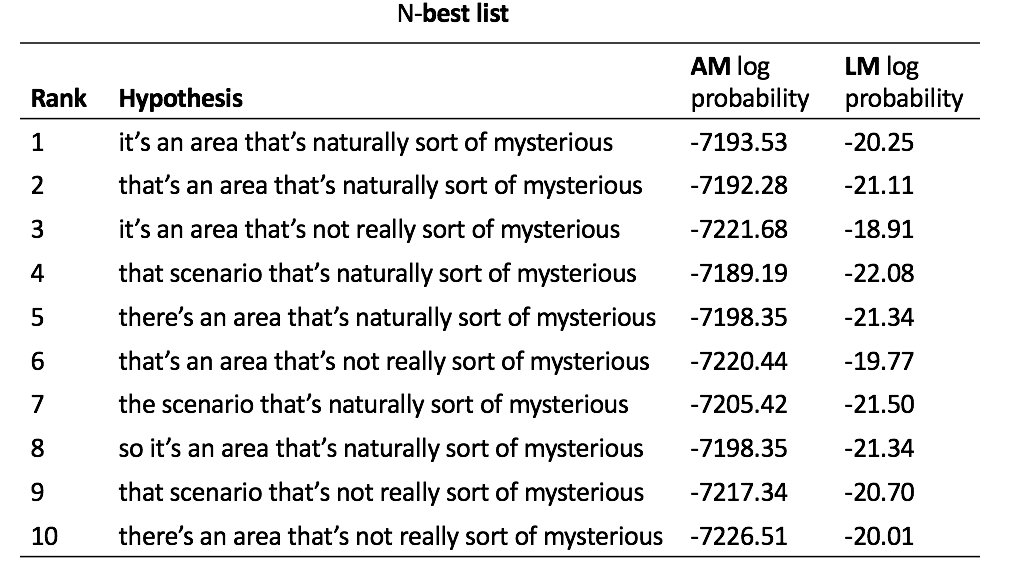
\includegraphics[width=1.0\textwidth]{struclm/nbest}
\end{figure}
\begin{figure}[htbp!]
\centering
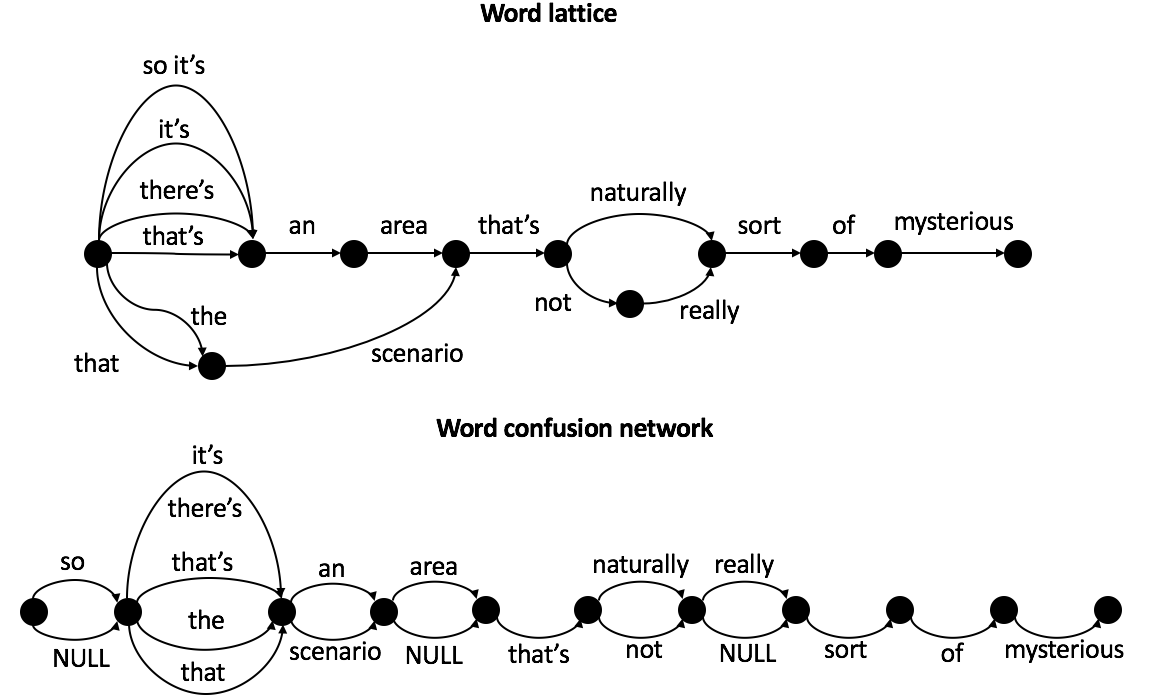
\includegraphics[width=1.0\textwidth]{struclm/wcn}
\caption{N-best列表、词格、词混淆网络是常见的总结了各种备选句子及其后验概率的结构。这些例子引用自\cite{jurafsky2014speech}。}
\label{fig:asr-output}
\end{figure}

语音识别的解码器可以输出词格或者词混淆网络作为中间结果。词格(word lattice)和词混淆网络(word confusion network)就提供了信息量更大的词识别的后验分布,而不像N最佳假设那样裁剪了得分较低的词。词格是一种可以高效地编码多种可能的词序列的有向图结构\cite{murveit1993large},如图~\ref{fig:asr-output}所示。所有可能的词序列就是每一条从开始结点到终结点的路径。另外,图中没有显示的信息还包括每条边的权值以及每个词的开始时刻和结束时刻信息。类似词格,词混淆网络也是一个可以枚举所有可能路径的有序图,不同的是它的结构有更多的限制。如图\ref{fig:asr-output}所示,词混淆网络由一个结点序列组成,每个结点表示的是词边界,且连续的两个结点之间由一些互斥的词连接。需要注意的是从词格转换成词混淆网络时会有一些额外的路径产生,比如图~\ref{fig:asr-output}中“\emph{the scenario area}”在词混淆网络有但不在词格中出现。然而,词格中的路径都会同时存在于词混淆网络中。此外,词混淆网络中还引入了空边\emph{NULL},用于表示与具体词无关的结点转移。

因为本工作研究的主要是循环神经网络自身的优化,所以一般来说我们都是先用一个基线的N-gram模型让语音识别解码器生成一个N-best列表,然后用循环神经网络对其进行重估计,用新模型的分数替换原本的分数,重排序,然后再重新对得分最高的假设句进行WER计算。



\section{N-gram语言模型}

\subsection{N-gram的概念}
N-gram是一种基于概率的语言模型,广泛应用于概率、通信理论、计算语言学。
根据语言模型的公式可知,当前单词出现的概率依赖于前面的历史,一直到第一个单词。
然而直观理解一下,很早的单词因为距离当前单词距离足够远,以至于影响近乎为零;并且如果一直考虑到第一个单词,会导致参数空间过大,时空复杂度过大,对计算资源造成严重浪费。
因此我们考虑在计算一个单词出现概率的时候
只考虑距离最近的N个历史,如图\ref{fig:ngram}所示,

\begin{figure}[!htbp]
  \centering
  \begin{minipage}[b]{0.6\textwidth}
    \captionstyle{\centering}
    \centering
    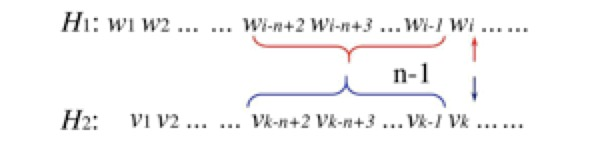
\includegraphics[width=\linewidth]{lm/ngram.jpeg}
    \bicaption[fig:ngram]{N-gram 结构}{N-gram structure}{Fig}{N-gram 结构}
  \end{minipage}     
\end{figure}


我们将历史映射到等价类S中,则得到当前单词出现的概率公式\ref{fig:wordp},

\begin{equation}
\begin{split}
	\label{eq:wordp}
   	S({w_1},{w_2},...,{w_i}) &= S({v_1},{v_2},...,{v_k}) \\
    iff  \quad H_1:(w_{i-n+2},...,{w_i}) &= H_2(w_{k-n+2},...,{w_k}) \\
	P({w_i}|{w_1},{w_2},...,{w_{i - 1}}) &= P({w_i}|S({w_1},{w_2},...,{w_{i - 1}}))
\end{split}
\end{equation}

考虑到整个句子,其N-gram语言模型概率计算如公式\ref{fig:ngram},
\begin{equation}
	\label{eq:ngram}
   	P(S) = \prod\limits_{i = 1}^N {P( {{w_i}|w_{i - n + 1}^{i - 1}} )}
\end{equation}
当$n=2$和$n=3$时分别称为bigram和trigram。


\subsection{数据平滑技术}
当数据匮乏或稀疏时,会导致很多词的概率预测为零,大规模数据统计方法与有限的训练语料之间必然产生数据稀疏问题,对于这种零概率问题,我们用到数据平滑技术去解决它们。
其基本思想是:在保证概率和为1的情况下,降低已出现n-gram条件概率分布,以使未出现的n-gram条件概率分布非零。

目前数据平滑的技术有很多,它是构造高鲁棒性语言模型的重要手段。
且数据平滑的效果与训练语料库的规模有关。
训练语料库规模越小,数据平滑的效果越显著;训练语料库规模越大,数据平滑的效果越不显著,甚至可以忽略不计。


\subsection{N-gram的扩展}
N-gram语言模型衍生出了一些变种,简单介绍一下:
1)	Class-based N-gram Model\cite{brown1992class}是按照词的分类建立语言模型,可以有效缓解数据稀疏问题。
它在语言模型训练的时候将单词以某种规则分成不同的类,可以让部分出现很少的单词不至于无法识别以致概率接近零,另一方面且可以方便融合部分语法信息,同时还能解决OOV(out of vocabulary)导致PPL偏高的问题。

2)	Topic-based N-gram Model将训练集按主题划分成多个子集,并对每个子集分别建立N-gram语言模型,例如采用狄利克雷混合作为参数的多项式分布估计的方法\cite{gildea1999topic},以解决语言模型的主题自适应问题。
按照划分主题,可以有效降低语言模型的PPL。

3)	Cache-based N-gram Model是一种新颖的语言模型,该模用一种缓存组件模式反映短期单词使用的情况\cite{kuhn1990cache},即利用cache缓存前一时刻的信息,以用于计算当前时刻概率,为语言模型加入历史信息,以解决语言模型动态自适应问题。

4)	Skipping N-gram Model和Trigger-based N-gram Mode从名字可以发现,一改N-gram忽略远距离相关性的弊端,因为可能当前单词的预测会与较远时刻曾经出现过的那次发射概率有关。
两者核心思想都是刻画远距离约束关系。


\subsection{N-gram的优劣}
N-gram模型的最主要的优势就是编码简单和训练快速。因为抽象来说只需要将训练数据过一遍,然后将信息和概率都存起来,就完成了。这方便不过多赘述。

但是缺点也很明显。首先,N元组对长距离的上下文关系的建模就很有问题,如“我 吃饭 之后 不喜欢 \textbf{洗碗}”,这里的“洗碗”这个词如果考虑到上下文里“吃饭”的信息就很容易作预测,但假设我们用的是三元组模型的话,模型只会考虑“不 喜欢”这个上下文,“洗碗”就无从谈起了。

另外,在N-gram语言模型中,词与词之间是“离散”的,举个例子,“周三”和“周四”两个词我们都知道是很相似的词,然而, 但在N-gram语言模型中,两个词却毫无联系,N-gram模型只是统计了元组在数据中出现的次数。因此,可能“语文课“ 定在 周三”得到的概率比较高(假设这句话数据中出现了多次),但“语文课 定在 周四”得到的概率就很低(如果这句话出现次数非常少的话)。

除此之外,N-gram还有着巨大的参数量,且随着N-gram中N的增加,参数量成指数级增加,而当N比较小时语言模型的性能又收到影响。 b n


%%%%%%%%%%%%%%%%%%%%%%%%%%%%%%%%%%%%%%%%%%%%%%%%%%%%%%%%%%%%%%%%

\section{循环神经网络语言模型RNNLM}

\subsection{人工神经网络}
人工神经网络是一种模仿生物神经网络的激励传播的结构和功能的数学模型或者说计算模型,它由大量的人工神经元以某种方式进行连接和计算,在学术界也常直接简称为神经网络(neural network,NN)。

神经网络由大量的节点相互连接构成,这些节点被称为“神经元”,或“单元”。
每个节点实际上是一个运算单元,代表着一种特定的函数,称为激励函数(activation function)每个连接传递到节点的信息经过这些神经元就相当于进行了一次神经元所代表的函数的运算。

每两个节点间的连接都代表一个对于通过该连接信号的加权值,称之为权重(weight)或参数矩阵,这些参数矩阵代表着相当于人的神经网络的记忆功能,训练一个神经网络实质上是对这些权重不断修改不断完善的过程。
网络的输出则根据网络的连接方式、权重值和激励函数的不同而不同,从而组成了不同类型不同功能的神经网络。
每个神经网络自身通常都是对自然界某种算法或者函数的逼近,也可以说是对一种逻辑策略的表达。
每个神经元的结构示意如图\ref{fig:neure}所示,$x_1$到$x_n$为输入向量,$b$为偏置,$f$为激励函数,$t$为神经元输出。
\begin{figure}[!htbp]
  \centering
  \begin{minipage}[b]{0.6\textwidth}
    \captionstyle{\centering}
    \centering
    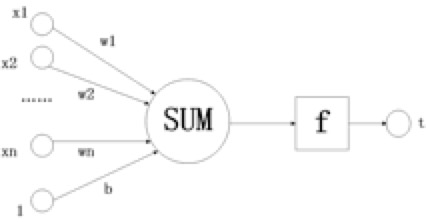
\includegraphics[width=\linewidth]{lm/neure.jpeg}
    \bicaption[fig:neure]{神经元结构}{neure structure}{Fig}{神经元结构}
  \end{minipage}     
\end{figure}
神经网络也分为单层神经网络和多层神经网络,后面我们研究涉及到的都是多层神经网络。
神经网络的种类有很多:前馈神经网络、循环神经网络(RNN)、卷积神经网络等。

多层神经网络也称深度神经网络(DNN),是一种前馈神经网络\cite{yu2011improved},是多层神经网络。它除了输入层和输出层,还有两个或两个以上的隐层,“深度”这个名字就体现在它有很多层上,其结构示意图如图\ref{fig:dnn}所示,
\begin{figure}[!htbp]
  \centering
  \begin{minipage}[b]{0.6\textwidth}
    \captionstyle{\centering}
    \centering
    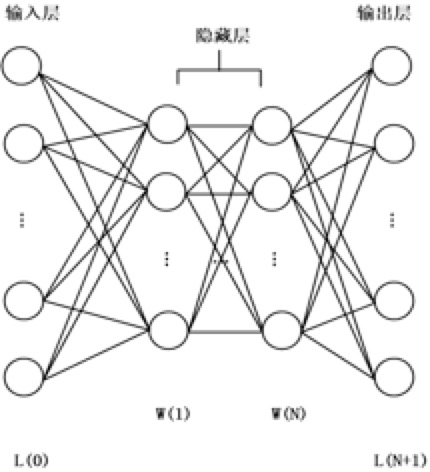
\includegraphics[width=\linewidth]{lm/dnn.jpeg}
    \bicaption[fig:dnn]{DNN结构}{DNN structure}{Fig}{DNN结构}
  \end{minipage}     
\end{figure}
神经网络语言模型是当今最成功的统计类语言模型,他们可以被广泛地应用于各种机器学习任务。
后文中本文主要使用的RNN和LSTM网络也和DNN类似,如果是深层的结构,则是基于此模型的。




\subsection{RNNLM的结构与原理}

不同于上文所介绍的前馈神经网络语言模型,本章所要研究的循环神经网络语言模型RNNLM和前馈神经网络语言模型之间最主要的区别就是历史的表现:前馈神经网络语言模型中对当前单词有影响的历史仅仅是当前句子它前面的几个单词,而RNNLM中对当前单词有效的历史是整个训练过程中出现过的所有单词。原因是RNNLM中的隐藏层代表着所有前面出现过的历史,而不仅仅是当前句子,因此这个模型可以从理论上代描绘足够长的历史信息,从而使对单词及句子的预测准确度提升。


下面介绍RNNLM的网络结构,假设本文所涉及的RNNLM都是只有一个隐藏层的RNNLM,如图\ref{fig:rnn}所示:
\begin{figure}[!htbp]
  \centering
  \begin{minipage}[b]{0.6\textwidth}
    \captionstyle{\centering}
    \centering
    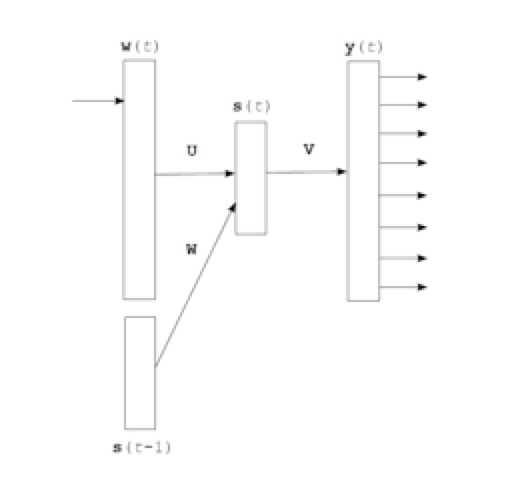
\includegraphics[width=\linewidth]{lm/rnn.jpeg}
    \bicaption[fig:rnn]{RNN结构}{RNN structure}{Fig}{RNN结构}
  \end{minipage}     
\end{figure}
$w$、$s$和$y$都是向量,$U$、$W$和$V$都是矩阵。$w$为当前时刻t的输入层向量,代表当前单词的编码,编码规则是:若当前单词在词典中的标号为$x$,则w向量中第x维为$1$,其他都是$0$,$x$的大小等于词表大小;$s(t-1)$是$t-1$时刻的神经网络的隐藏层的输出;$s(t)$为当前的隐藏层,其计算方法如公式\ref{eq:sj}所示;$y(t)$是当前t时刻的输出层,代表t+1时刻每个单词在当前历史下的概率,即$P({w_t+1}|{w_t}, s(t-1))$,计算公式如公式\ref{eq:yk}所示;矩阵$U$和$W$是在输入层到隐藏层之间,$V$是从隐藏层到输出层之间的矩阵。
\begin{equation}
	\label{eq:sj}
   	{s_j}\left( t \right) = f\left( {\sum\limits_i {{w_i}\left( t \right){u_{ji}} + \sum\limits_l {{s_l}\left( {t - 1} \right)} } {w_{jl}}} \right)
\end{equation}
\begin{equation}
	\label{eq:yk}
   	{y_k}\left( t \right) = g\left( {\sum\limits_j {{s_j}\left( t \right){v_{kj}}} } \right)
\end{equation}
上面的公式还能更简单地写成矩阵运算的形式:
\begin{equation}
\label{eq:st}
   	s\left( t \right) = f\left( {Uw\left( t \right) + Ws\left( {t - 1} \right)} \right)
\end{equation}
\begin{equation}
\label{eq:yt}
   	y\left( t \right) = g\left( {Vs\left( t \right)} \right)
\end{equation}
其中$f(x)$和$g(x)$分别为sigmoid激活函数和softmax激活函数。下面分别介绍一下这两个公式的意义、求导及作用:
a)	sigmoid函数的公式与求导如公式\ref{eq:sigmoid}所示:

\begin{equation}
\begin{split}
	\label{eq:sigmoid}
   		f\left( x \right) &= \frac{1}{{1 + {e^{ - x}}}}\\
		f'\left( x \right) &= f\left( x \right)\left( {1 - f\left( x \right)} \right)
\end{split}
\end{equation}


\ref{fig:rnn}所示:
\begin{figure}[!htbp]
  \centering
  \begin{minipage}[b]{0.6\textwidth}
    \captionstyle{\centering}
    \centering
    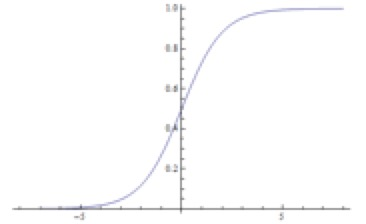
\includegraphics[width=\linewidth]{lm/sigmoid.jpeg}
    \bicaption[fig:sigmoid]{sigmoid结构}{sigmoid structure}{Fig}{sigmoid结构}
  \end{minipage}     
\end{figure}

函数图像如图\ref{fig:sigmoid}所示,结合图\ref{fig:neure}的神经元结构,其f函数即为求隐藏层$s$的sigmoid函数,我们将输入层神经元的输入表示为${x_1}-{x_n}$,输出层为$y$,$b$为偏置,则每一个神经元的计算过程可用公式\ref{eq:sigmoid2}表示。
\begin{equation}
	\label{eq:sigmoid2}
   	y = sigmoid\left( {\sum\limits_i {{x_i} + b} } \right)
\end{equation}
	Sigmoid函数相加可以模拟任何非线性函数,来表示语言模型的计算。
    
    
b)	softmax激活函数的公式如公式\ref{eq:gxm}所示,隐层的输出和矩阵$V$进行矩阵相乘后通过softmax函数得到输出层的发射概率。其中假设$x$为softmax函数的输入,输出为$g$。
\begin{equation}
	\label{eq:gxm}
   	g\left( {{x_m}} \right) = \frac{{{e^{{x_m}}}}}{{\sum\limits_k {{e^{{x_k}}}} }}
\end{equation}

上文提到过,输出层的发射概率向量指的是从$0$时刻一直到$t$时刻以当前为历史的下一个单词的概率,如$y_i$指的是下一个单词是此表中的标号为$i$的单词出现的概率。而直观上理解softmax激活函数的意义是将输出层的输出形式转换成一个有效的概率分布,即输出向量的所有元素都大于$0$,并且和为$1$。


\subsection{RNNLM的练流程和步骤}


结合上面的RNNLM的结构图,需要强调RNNLM需要学习的是输入层和隐藏层之间的矩阵$U$、$W$以及隐藏层到输出层之间的矩阵$V$,而并不是那些神经元,神经元只是完成计算功能的单位。知道了这一点之后,可以归纳出RNNLM的训练流程:如图\ref{fig:rnnflow}所示。

\begin{figure}[!htbp]
  \centering
  \begin{minipage}[b]{0.6\textwidth}
    \captionstyle{\centering}
    \centering
    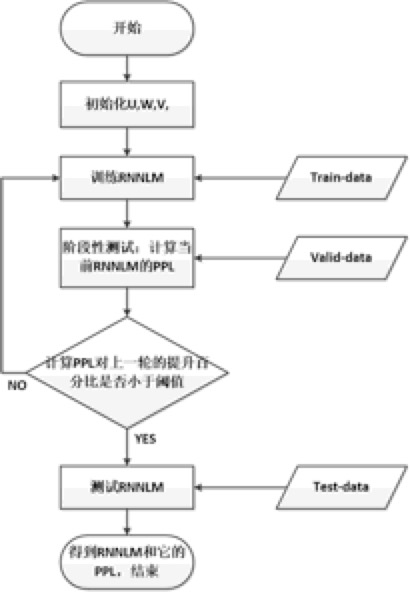
\includegraphics[width=\linewidth]{lm/rnnflow.jpeg}
    \bicaption[fig:rnnflow]{RNNLM训练流程}{RNNLM training process}{Fig}{RNNLM训练流程}
  \end{minipage}     
\end{figure}

首先对RNNLM进行初始化,即$U$、$W$和$V$的初始化,我们采取的方式是随机初始化,对矩阵中的每个元素随机一个$0$至$0.1$之间的实数;接着我们将训练集输入到神经网络中训练这三个矩阵,得到第一轮的训练结果;这时我们用valid集合去计算当前RNNLM的混淆度(PPL)和上一轮的结果比较(至少训练两轮,第一轮不比较),看PPL提升的程度是多少,若小于一定的数值则说明当前RNNLM已经趋于稳定,继续训练下去基本上对它没有改变,这时退出训练过程,得到最终的RMMLM;最后我们参考前面用valid集测试语言模型的方法,用test集对其进行测试,测出来的PPL即为最后的PPL。
对于第二步训练RNNLM有多轮训练,其某一轮训练的具体的训练步骤如图\ref{fig:rnnstep}所示。

(1)设置一个时间计数器$t$,初始$t=0$,初始化隐藏层神经元的状态,令其为$1$。

(2)把时间计数器$t$的值增加$1$。

(3)更具当前的单词wt处理出当前输出层的向量$w(t)$,具体方法是:初始化一个大小为的每一维都为$0$的向量, 是词表的大小;求出当前单词$w_t$在词表中的序号$p$,将$w(t)$的第$p$维置为$1$。

(4)将上一时刻,即$t-1$时刻的隐藏层向量$s(t-1)$复制储存,作为这时刻的输入。

(5)执行神经网络的前向传播得到隐藏层$s(t)$和输出层$y(t)$,
前向传播的具体方法是:
首先输入层$w(t)[1*{v_s}]$与矩阵$U[{v_s}*{h_s}]$进行矩阵相乘的结果中间向量${s_1}[1*{h_s}]$与上一轮隐藏层$s(t-1)[1*{h_s}]$与矩阵$W[{h_s}*{h_s}]$进行矩阵相乘得到中间向量$s2[1*{h_s}]$;然后将中间向量$s_1$与中间向量$s_2$相加得到当前$t$时刻的隐藏层$s(t)$;最后将$s(t)[1*{h_s}]$与矩阵$V({h_s}*{v_s})$进行矩阵相乘得到输出层向量$y(t)[1*{v_s}]$。

(6)计算输出层的梯度误差$e(t)$。

(7)反向传播输出层的梯度误差$e(t)$依次到输出层与隐藏层之间的矩阵$V$、隐藏层$s(t)$、输入层到隐藏层之间的矩阵$U$和$W$,并根据梯度误差和学习率修改它们。

(8)判断是否所有的训练数据都被处理过了,如果是则跳出循环,否则转到步骤(2)。


\begin{figure}[!htbp]
  \centering
  \begin{minipage}[b]{0.6\textwidth}
    \captionstyle{\centering}
    \centering
    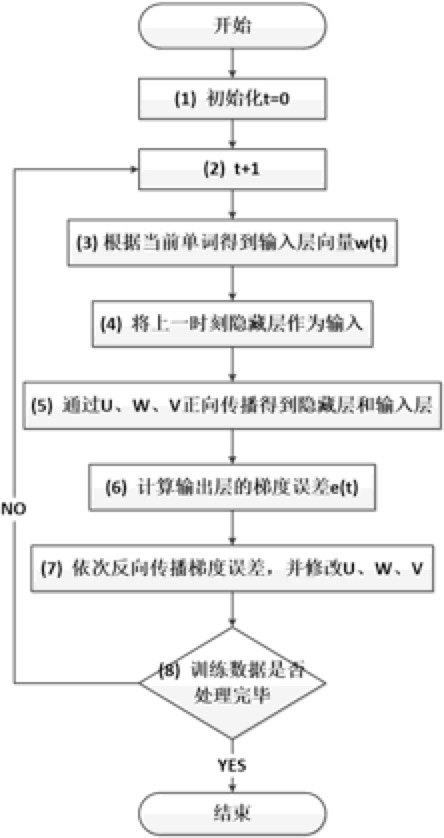
\includegraphics[width=\linewidth]{lm/rnnstep.jpeg}
    \bicaption[fig:rnnstep]{RNNLM训练步骤}{RNNLM training steps}{Fig}{RNNLM训练步骤}
  \end{minipage}     
\end{figure}


\subsection{RNNLM的训练数学基础及BPTT}
\subsubsection{普通反向传播(BP)}
要把循环神经网络中的基于时间的反向传播算法讲清楚,我们首先要介绍DNN中的普通的反向传播。见DNN的结构图\ref{fig:dnn},其具有多个隐层,反向传播的思想就是先求出输出层的梯度误差,然后每一个隐藏层的梯度误差都可以根据其后面一层的隐藏层的梯度误差得到;得到梯度误差后,我们可以根据微分的方法求出待求参数的梯度,根据梯度误差、梯度、和学习率对当前参数进行更新。
首先我们需要求输出的损失函数,在分类器中最长见的损失函数是负似然对数函数(negative log-likelihood),如图\ref{fig:rnn}在输出层我们会对输出向量进行softmax操作,因此我们可以将损失函数写成公式\ref{eq:loss}的形式:
\begin{equation}
	\label{eq:loss}
   	L\left( \theta  \right) =  - \sum\limits_{i = 1}^T {\log \left( {P\left( {s = {t_i}|{o_i}} \right)} \right)} 
\end{equation}
损失函数也被称为交叉熵
我们可以推断出损失函数对输出层的偏导数公式如公式\ref{eq:eot}:
\begin{equation}
\begin{split}
\label{eq:eot} 	
	{e_o}\left( t \right) &= \frac{{\partial L}}{{\partial {y_i}^{L + 1}}}{\rm{ }} = {\rm{ }}{{ - \partial \log \left( {\frac{{{e^{{y_t}^{L + 1}}}}}{{\sum\limits_i {{e^{{y_i}^{L + 1}}}} }}} \right)} \mathord{\left/
	 {\vphantom {{ - \partial \log \left( {\frac{{{e^{{y_t}^{L + 1}}}}}{{\sum\limits_i {{e^{{y_i}^{L + 1}}}} }}} \right)} {\partial {y_t}^{L + 1}}}} \right.
 \kern-\nulldelimiterspace} {\partial {y_t}^{L + 1}}}\\
	&=  \frac{{{e_i}^{L + 1}}}{{\sum\limits_i {{e^{{y_i}^{L + 1}}}} }} - \frac{{\partial {y_t}^{L + 1}}}{{\partial {y_i}^{L + 1}}}\\
	&=  P\left( {s = i|o} \right) - [t = i]
\end{split}
\end{equation}

	我们令$d(t)$表示代表第$t+1$个单词(待预测单词)的目标向量,即$w(t+1)$在词表中的标号的那一维为$1$,其它维数都为$0$;$y(t)$为输出层的输出,可以得到公式\ref{eq:eot2}:
\begin{equation}
	\label{eq:eot2}
   	{e_o}\left( t \right) = d\left( t \right) - y\left( t \right)
\end{equation}
因为非常碰巧的损失函数对输出层的偏导数的表现形式为期待的正确向量与概率预测向量之间的差,所以也被称为梯度误差或error。


接着分析输出层的梯度误差是如何传递的。如图\ref{fig:dnnbp}所示:
\begin{figure}[!htbp]
  \centering
  \begin{minipage}[b]{0.6\textwidth}
    \captionstyle{\centering}
    \centering
    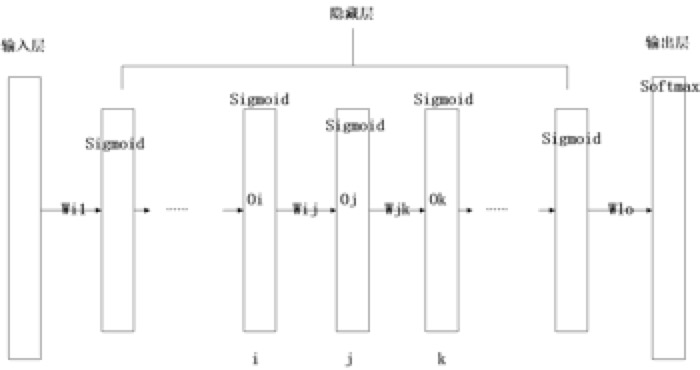
\includegraphics[width=\linewidth]{lm/dnnbp.jpeg}
    \bicaption[fig:dnnbp]{DNN的反向传播}{DNN back propagation}{Fig}{DNN反向传播}
  \end{minipage}     
\end{figure}

在DNN中假设相邻的三个隐藏层的标号分别为$i$、$j$、$k$(比$l-1$,$l$,$l+1$表示更易于区分),$o_i$、$o_j$、$o_k$分别是隐藏层$i$、$j$、$k$的输出(output)向量, ${w_ij}$是$i$层到$j$层之间的矩阵,${w_jk}$是$j$层到$k$层之间的矩阵。正在推导公式之前先要介绍一下多元复合函数求导的链式法则,首先有个函数$f({x_1},...,{x_n})$并且对于每个$x_i$有${x_i={g_i}({u_1},...,{u_m})}$,并且所有函数都是可导的,则有公式\ref{fui}。
\begin{equation}
	\label{eq:fui}
   	\frac{{\partial f}}{{\partial {u_i}}} = \sum\limits_j {\frac{{\partial f}}{{\partial {x_j}}} \cdot \frac{{\partial {g_j}}}{{\partial {u_i}}}} 
\end{equation}
首先,我们求损失函数关于${w_ij}$的偏导数,采用上述的链式法则,如公式\ref{lwij}。
\begin{equation}
	\label{eq:lwij}
 	\begin{split}
\frac{{\partial L}}{{\partial {w_{ij}}}} &4= \frac{{\partial L}}{{\partial {o_j}}} \cdot \frac{{\partial {o_j}}}{{\partial {w_{ij}}}}\\
&= \frac{{\partial L}}{{\partial {o_j}}} \cdot {o_j} \cdot \left( {1 - {o_j}} \right) \cdot {o_i}\\
\because \quad {o_j} &= sigmoid({o_i}\cdot{w_ij} + bias)\\
\therefore \quad {o_j}‘ &= {o_j} \cdot (1-{o_j})
\end{split}
\end{equation}


我们定义前面一部分为第$j$层的梯度误差,如公式\ref{eq:drj}
\begin{equation}
	\label{eq:erj}
   	er{r_j} = \frac{{\partial L}}{{\partial {o_j}}} \cdot {o_j} \cdot \left( {1 - {o_j}} \right)
\end{equation}

然后可以求得${w_ij}$的梯度为${err_j}*{o_i}$。

正向传播时我们是按箭头的方向,将和$o_i$和${w_ij}$进行矩阵相乘后经过神经元的sigmoid函数,$o_i$为作为第$j$层的输出,反向传播我们则反过来,现在求出$err_j$后,我们来看$err_j$和第$k$层的$err_k$有什么关系,继续用复合函数的链式法则,得出公式\ref{eq:errj}。
\begin{equation}
	\label{eq:errj}
   	\begin{split}
er{r_j}&{\rm{ }} = \frac{{\partial L}}{{\partial {o_j}}} \cdot {o_j} \cdot \left( {1 - {o_j}} \right)\\
&{\rm{         = }}\sum\limits_{k = 1}^{hiddensize} {\left( {\frac{{\partial L}}{{\partial {o_k}}} \cdot \frac{{\partial {o_k}}}{{\partial {o_j}}}} \right)}  \cdot {o_j} \cdot \left( {1 - {o_j}} \right)\\
&{\rm{         = }}\sum\limits_{k = 1}^{hiddensize} {\left( {\frac{{\partial L}}{{\partial {o_k}}} \cdot {o_k} \cdot \left( {1 - {o_k}} \right) \cdot {w_{jk}}} \right)}  \cdot {o_j} \cdot \left( {1 - {o_j}} \right)\\
&{\rm{         = }}\sum\limits_{k = 1}^{hiddensize} {\left( {er{r_k} \cdot {w_{jk}}} \right)}  \cdot {o_j} \cdot \left( {1 - {o_j}} \right)\\
\because \quad {r_k}&{\rm{ }} = \frac{{\partial L}}{{\partial {o_k}}} \cdot {o_k} \cdot \left( {1 - {o_k}} \right)\\
\end{split}
\end{equation}

            
结合RNN的结构图\ref{fig:rnn},只有一个隐藏层,我们根据上述公式去更新矩阵$V$、$U$、$W$。我们可以根据输出层的梯度误差得到隐藏层和输出层之间的矩阵V的更新方式,如公式\ref{eq:vjk}通过输出层的梯度误差对其进行更新。
\begin{equation}
	\label{eq:vjk}
   	{v_{jk}}\left( {t + 1} \right) = {v_{jk}}\left( t \right) + {s_j}\left( t \right){e_{ok}}\left( t \right)\alpha 
\end{equation}

其中$\alpha$是学习率,学习率会随着训练的轮次一轮一轮递减。公式中$j$从$1$循环到隐藏层的大小 ,$k$从$1$循环到输出层大小。${s_j}(t)$是当前$t$时刻的隐藏层的第$j$个神经元的输出,${e_ok}(t)$是当前时刻输出层第$k$个神经元的梯度误差。接下来我们用L2归一化方法得到公式\ref{eq:vjk2}。
\begin{equation}
	\label{eq:vjk2}
   {v_{jk}}\left( {t + 1} \right) = {v_{jk}}\left( t \right) + {s_j}\left( t \right){e_{ok}}\left( t \right)\alpha  - {v_{jk}}\left( t \right)\beta 
\end{equation}

其中$\beta$是归一化参数。归一化是为了防止过拟合而采用的,根据实验结果和前人论文经验,后面实验数据所采用的$\beta$都是$10^{-6}$,公式\ref{eq:vjk2}还能写成矩阵相乘的形式如公式\ref{eq:vjk3}。
\begin{equation}
	\label{eq:vjk3}
   	V\left( {t + 1} \right) = V\left( t \right) + s\left( t \right){e_o}{\left( t \right)^T}\alpha  - V\left( t \right)\beta 
\end{equation}

隐藏层的梯度误差可以写成公式\ref{eq:eht}的形式,其中表示矩阵乘法
\begin{equation}
	\label{eq:eht}
   	\begin{split}
{e_h}\left( t \right) &= {d_h}\left( {{e_o}{{\left( t \right)}^T}V,t} \right)\\
{d_{hj}}(x,t) &= x{s_j}\left( t \right)\left( {1 - s\left( j \right)} \right)
	\end{split}
\end{equation}

同样的根据上文推导出来的求梯度公式,我们得到了隐藏层的梯度误差${e_h}(t)$可以得出更新输入层和隐藏层之间的矩阵U的公式\ref{eq:uij},
\begin{equation}
	\label{eq:uij}
   	{u_{ij}}\left( {t + 1} \right) = {u_{ij}}\left( t \right) + {w_i}\left( t \right){e_{hj}}\left( t \right)\alpha  - {u_{ij}}\left( t \right)\beta 
\end{equation}

写成矩阵相乘的形式:
\begin{equation}
	\label{eq:ut+1}
	U\left( {t + 1} \right) = U\left( t \right) + w\left( t \right){e_h}{\left( t \right)^T}\alpha  - U\left( t \right)\beta 
\end{equation}

需要注意的是,在当前t时刻,只有一个神经元是活跃的,当输入向量为$w(t)$的时候,$w(t)$中为$0$的元素所连接的w都是不会改变的,因此在程序中实现更新的时候只用更新$w(t)$为$1$的那个元素对应的一列$U$矩阵的权值,这样可以达到提高速度的目的。当前的$W$矩阵修改为\ref{eq:ut+1}:
\begin{equation}
	\label{eq:sigmoid2}
	{w_{lj}}\left( {t + 1} \right) = {w_{lj}}\left( t \right) + {s_l}\left( {t - 1} \right){e_{hj}}\left( t \right)\alpha  - {w_{lj}}\left( t \right)\beta 
\end{equation}
	
写成矩阵相乘的形式为\ref{eq:wt+1}
\begin{equation}
	\label{eq:wt+1}
   	W\left( {t + 1} \right) = W\left( t \right) + {s_l}\left( {t - 1} \right){e_{hj}}{\left( t \right)^T}\alpha  - W\left( t \right)\beta 
\end{equation}


\subsubsection{基于时间的反向传播算法(BPTT)}
上文所介绍的训练算法是普通的反向传播算法,一般用于DNN训练中,虽然RNN的训练和普通的只有一层隐藏层的前馈网络(包括DNN)是一样的,但是唯一的不同是RNN结构中输入层不仅是当前单词的表示向量,还包括上一步或者说上一个时刻训练得到的隐藏层。 


然而,可以发现这样的训练方法并不是最优的,因为神经网络试图根据当前的视神经网络状态和当前的单词去尽量正确的预测下一个单词,但是当前隐藏层储存的实际上有用信息太少了,因为只有一个隐藏层,就算有多个隐藏层,它也是有限的。所以如果这个神经网络可以记忆更多的前后文信息,并将它们储存在隐藏层中,预测的准确率就会高很多。

\begin{figure}[!htbp]
  \centering
  \begin{minipage}[b]{0.6\textwidth}
    \captionstyle{\centering}
    \centering
    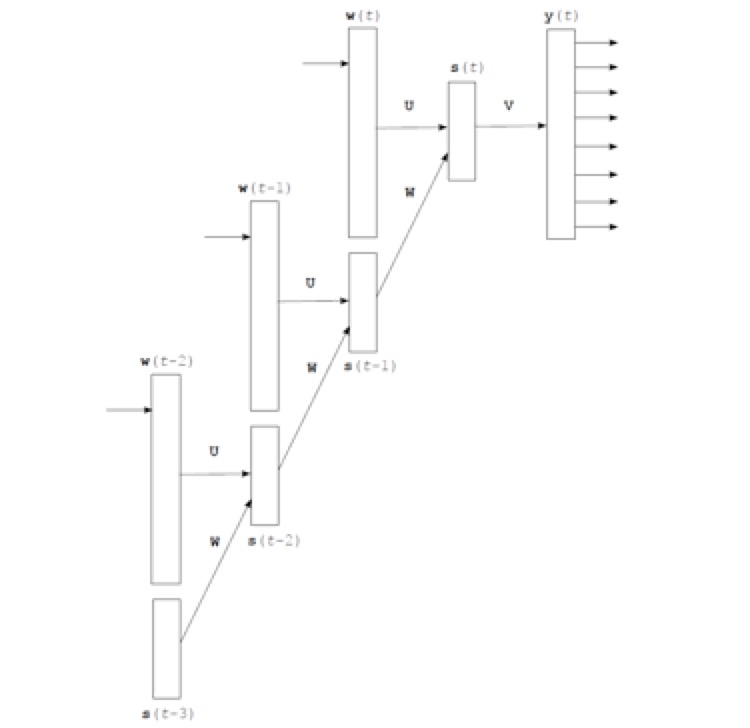
\includegraphics[width=\linewidth]{lm/bptt.jpeg}
    \bicaption[fig:bptt]{BPTT结构图}{RNNLM BPTT structure}{Fig}{BPTT结构图}
  \end{minipage}     
\end{figure}

因此我们保持前向传播的算法不变,在反向训练通过梯度误差对网络参数进行修改的时候,对其结构进行一些调整:我们将只有一个隐藏层的RNN神经网络经过N个时间、完成N各步骤的过程看成是一个有N个隐藏层的神经网络,因为每一个时刻的隐藏层的维度相同,并且连接他们之间的W矩阵也是完全一样的,参见上文RNN结构图,上一时刻的隐藏层会作为而这一时刻的输出,再往前推更多的时刻,看起来就是一个DNN的结构。

如图\ref{fig:bptt}中的神经网络的训练方式可以按照常规的梯度下降的方法,梯度误差会从当前隐藏层$s(t)$依次传向$s(t-1$)、$s(t-2)$、$...$、$s(1)$,并依次更新当前误差所在层和前一次之间的权值矩阵(记作$W$),梯度误差的向前传递是一个递归的过程,写成如公式\ref{eq:eh}的形式
\begin{equation}
	\label{eq:eh}
   	{e_h}\left( {t - \tau  - 1} \right) = {d_h}\left( {{e_h}{{\left( {t - \tau } \right)}^T}W,t - \tau  - 1} \right)
\end{equation}
其中函数在公式\ref{eq:vjk}中定义了。

	但是这样的展开是无穷无尽的,前面出现过多少训练数据当前的BP就能向前展开多少层,但是梯度误差会随着传播的过程变得越来越小直到趋近于$0$,但是展开的层数越多所耗费的时间复杂度和空间复杂度就越大,因为耗费巨大时空代价去对$W$进行接近于$0$的修改是没有必要的,因此我们采取一种截断的BPTT,即向前展开有限层的BPTT,实验发现向前展开$5$层左右是比较好的。这就类似N-gram的语言模型算法,理论上要往前推到头,但是映射等价类的做法就好比这里的截断操作,我们在N-gram算法中常用到$4$-gram。
	结合图\ref{fig:bptt},U矩阵在BPTT中的学习公式为\ref{eq:uijt+1}:
    
\begin{equation}
	\label{eq:uijt+1}
   	{u_{ij}}\left( {t + 1} \right) = {u_{ij}}\left( t \right) + \sum\limits_{z = 0}^T {{w_i}\left( {t - z} \right){e_{hj}}\left( {t - z} \right)\alpha  - {u_{ij}}\left( t \right)\beta } 
\end{equation}

其中$T$是这个神经网络BPTT时向前展开的总层数,同样的,它也可以写成矩阵相乘的形式\ref{eq:ut+2}
\begin{equation}
	\label{eq:ut+2}
   	U\left( {t + 1} \right) = U\left( t \right) + \sum\limits_{z = 0}^T {w\left( {t - z} \right){e_h}{{\left( {t - z} \right)}^T}\alpha  - U\left( t \right)\beta } 
\end{equation}
十分需要注意的是,矩阵$U$的更新是一次性完成的,并不随着梯度误差的反向传播而递增,那样会导致训练的不稳定性。同样的,矩阵$W$的更新方式和$U$类似
\begin{equation}
	\label{eq:wlj}
   	{w_{lj}}\left( {t + 1} \right) = {w_{lj}}\left( t \right) + \sum\limits_{z = 0}^T {{s_l}\left( {t - z - 1} \right){e_{hj}}\left( {t - z} \right)\alpha  - {u_{lj}}\left( t \right)\beta } 
\end{equation}
写成矩阵相乘为\ref{eq:wt+2}
\begin{equation}
	\label{eq:wt+2}
   	W\left( {t + 1} \right) = W\left( t \right) + \sum\limits_{z = 0}^T {s\left( {t - z - 1} \right){e_h}{{\left( {t - z} \right)}^T}\alpha  - W\left( t \right)\beta } 
\end{equation}

通过上述公式,阐述了RNNLM在进行BPTT的时候的理论算法。


\section{长短时间记忆神经网络语言模型LSTMLM}
LSTM是循环神经网络的一种,它于1997年被Sepp Hochreiter and Jürgen Schmidhuber 提出cite{hochreiter1997long},和大部分的RNN一样,一个LSTM神经网络在给定了足够的网络单元时可以完成一台常见计算机可以完成的任何计算。但是不同于传统的RNN, LSTM更适合用于学习那些有很长一段时间滞后并且滞后时间的长短未知的重要事件,这也是为什么LSMT在有的方面比RNN,N-gram等语言模型算法更优秀的原因。例如,LSTM在不分段的连写识别中取得了最好的成绩\cite{graves2009novel},另外,LSTM神经网络也在自动语音识别中取得很好的成绩\cite{graves2013speech}。

训练一个LSTM神经网络同样用的是迭代梯度下降算法和基于时间的反向传播算法,然而在1991年突然意识到随着重要事件之间的间隔时间,误差梯度指数会迅速消失\cite{hochreiter1991untersuchungen}\cite{hochreiter2001gradient},然而,对于每一个LSTM块,当输出层的误差被计算算出来时,这个误差会被困在当前的记忆块中 ,这个记忆块会不断地传回错误直到切断这个值,这个BPTT的方法对于训练一个LSTM块去记住一个持续时间的值非常有效。

因为句子所具有的时序性,循环神经网络语言模型(RNNLM)作为一种有隐层自环的时序性神经网络模型,能够保存有历史信息并对其加以利用,打破了传统统计学语言模型的统治地位,并在短时间内发展迅速。其中,更有长短时间记忆(LSTM)单元替代传统的RNNLM中的隐层单元,以达到对更长历史信息的记忆和利用。其结构中有很多的门来控制对历史信息的记忆,公式如下:


在训练语言模型时,求损失函数对每个参数的偏导数即可得到梯度,接着利用梯度和步长(学习率)对模型参数进行更新。

\subsection{LSTM单元及其数学原理}

\subsection{LSTM的优劣}



